\documentclass[aps,pra,reprint,amsmath,amssymb]{revtex4-1}

\usepackage{subfigure,dcolumn}
\usepackage[T2A,T1]{fontenc}
\usepackage[english]{babel}

\usepackage{braket}
\usepackage{graphicx}
\usepackage[colorinlistoftodos]{todonotes}
\usepackage[utf8]{inputenc}

% The following package will be used to typeset the LaTeX codes and is not a necessity to this template
\usepackage{listings}
\lstloadlanguages{[LaTeX]TeX}
\lstset{language=[LaTeX]TeX,keywordstyle=\color{red},showspaces=true,breaklines=true,breakatwhitespace=true,basicstyle=\small\tt,commentstyle=\color{white},frame=single,framerule=0pt,backgroundcolor=\color{yellow}}


\begin{document}


\title{Causality and the N-photon Scattering matrix in waveguide QED}

\author{...}
\affiliation{...}
\email[Corresponding author, ]{The name, complete address, telephone number, and e-mail address of the author to whom correspondence and proofs should be sent.}


\begin{abstract}
The scattering matrix is one of the most fundamental objects for
describing particle processes. It connects the far past state with the
far future state, where the particles are well described by a free
Hamiltonian but they interact in some nontrivial way
for mid times. It can always be split into two parts: the linear part,
where each particle is scattered independently, and the nonlinear one,
which gives information about the interaction among the
particles. Here, we study the linear part of the scattering matrix for
$N$ photons impinging on a local system with several stable states. 
bla, bla
\end{abstract}


\keywords{Quantum optics, scattering matrix, and few-photon photonics.}

\maketitle


\section{Introduction}

{\color{blue}Blablabla on waveguide QED (wQED), scattering matrix as a fundamental object, and causality.} \cite{weinberg1995,Xu2016}


\section{Model in quantum photonics} 

{\color{blue}Hamiltonian and Fig. \ref{fig:input}.}

\begin{figure}
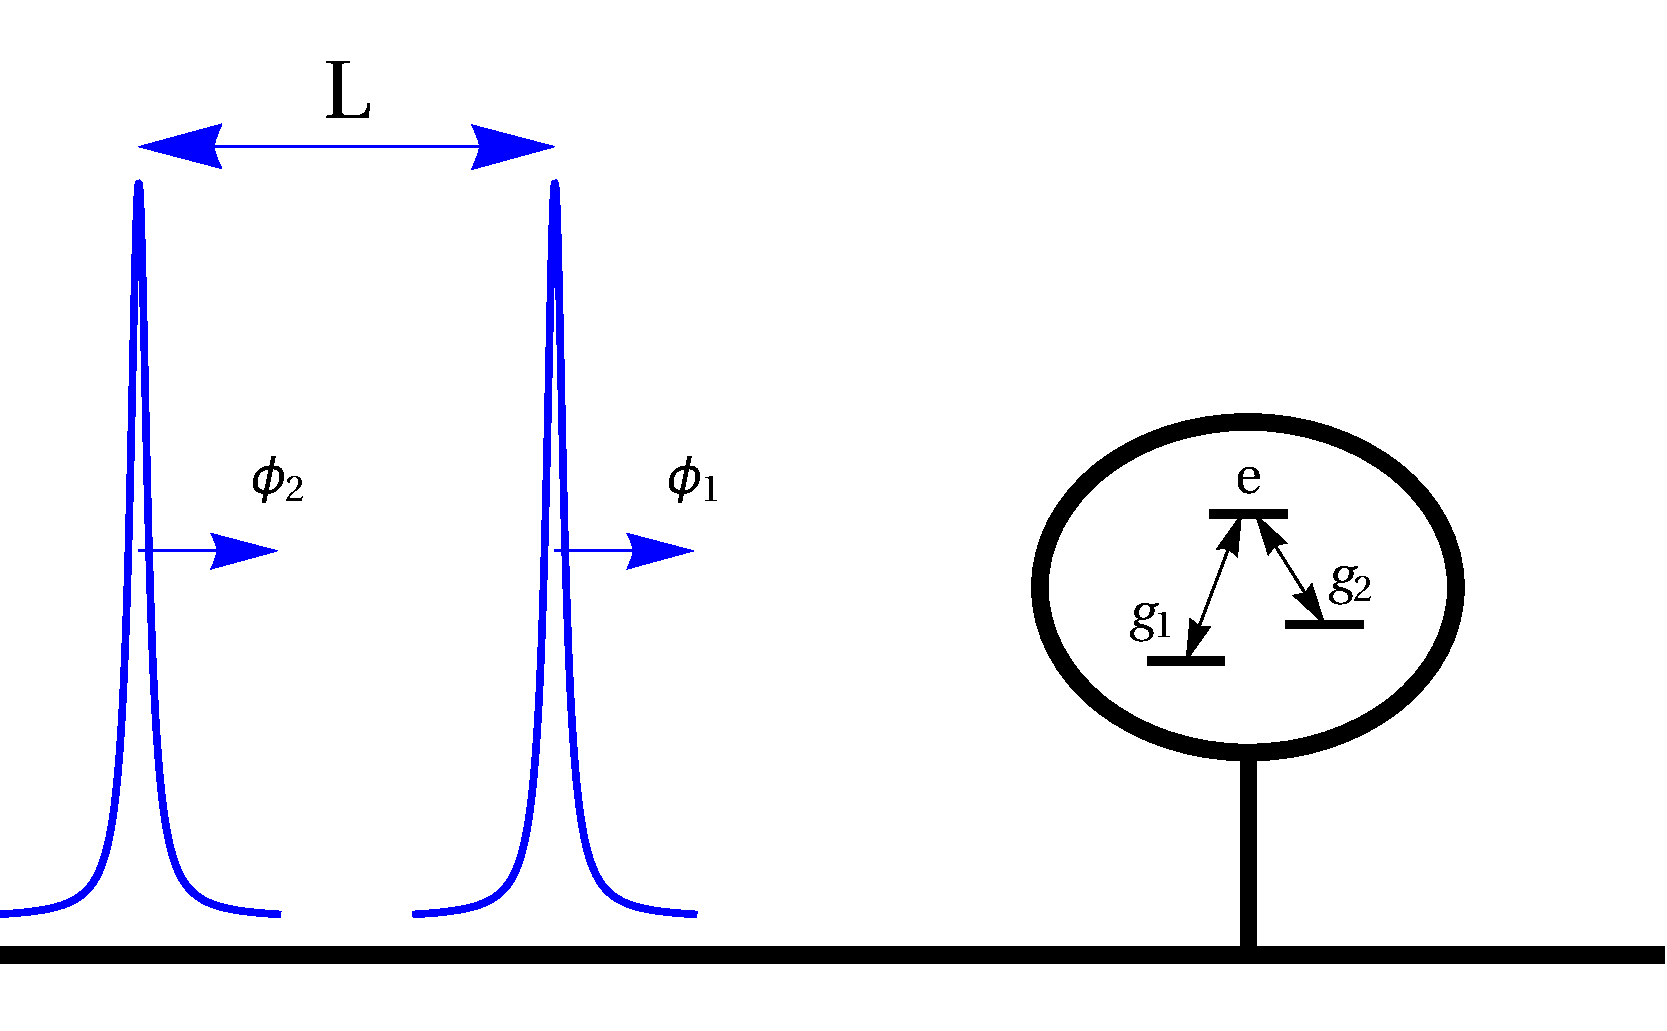
\includegraphics[scale=0.25]{input.pdf}
\caption{Two-photon input state impinging on a $\lambda$ atom. The state $e$ is an unstable state which decays to the stable ones, $g_1$ and $g_2$.}
\label{fig:input}
\end{figure}

\section{Free-field causality}

{\color{blue}Bounds for the commutators of the free theory.}

\section{Well-defined scattering}

{\color{blue}Conditions required for having well-defined scattering:

\begin{enumerate}
\item ground state $\simeq$ vacuum far enough from the scatterer,
\item free evolution for the fields far enough from the scatterer, and
\item Fig. with decaying ground state.
\end{enumerate}
}

\section{Cluster revisited}

{\color{blue}
Scattering amplitude between two distant events from the cluster principle: $A_{12\to 1'2'}^{\nu\to\mu} = \sum_\lambda A_{1\to 1'}^{\nu\to\lambda}A_{2\to 2'}^{\lambda\to\mu}$.
\begin{enumerate}
\item Build the ansatz for the scattering matrix in position space for $N$ photons using the cluster principle + step functions.
\item See the connection with the previous identity.
\item Conditions for the commutator $[a_\text{out}(t),a_\text{in}^\dagger(t')]$ so that $A_{12\to 1'2'}^{\nu\to\mu} = \sum_\lambda A_{1\to 1'}^{\nu\to\lambda}A_{2\to 2'}^{\lambda\to\mu}$ is true \cite{Xu2015}.
\end{enumerate}
}

\section{Examples}

{\color{blue}
\begin{enumerate}
\item $\lambda$ atom with $N=2$ in momentum space \cite{Xu2016}. Fluorescence from the new part of $S^0$. How the fluorescence decays.
\item Ultrastrong MPS. Fig. with resonance fluorescence. We might include a figure with the decay of the fluorescence as a function of $L$. \cite{Sanchez-Burillo2014,Sanchez-Burillo2015}.
\end{enumerate}
}

\section{Summary and acknowledgements}

\appendix

\section{$S^0$ in momentum space}

{\color{blue}
\begin{enumerate}
\item Computation in general: Figs. \ref{fig:lower} and \ref{fig:upper}.
\item To particularize for $N=2$ and $\lambda$ atom \cite{Xu2016}.
\end{enumerate}
}

\begin{figure}[tbh!]
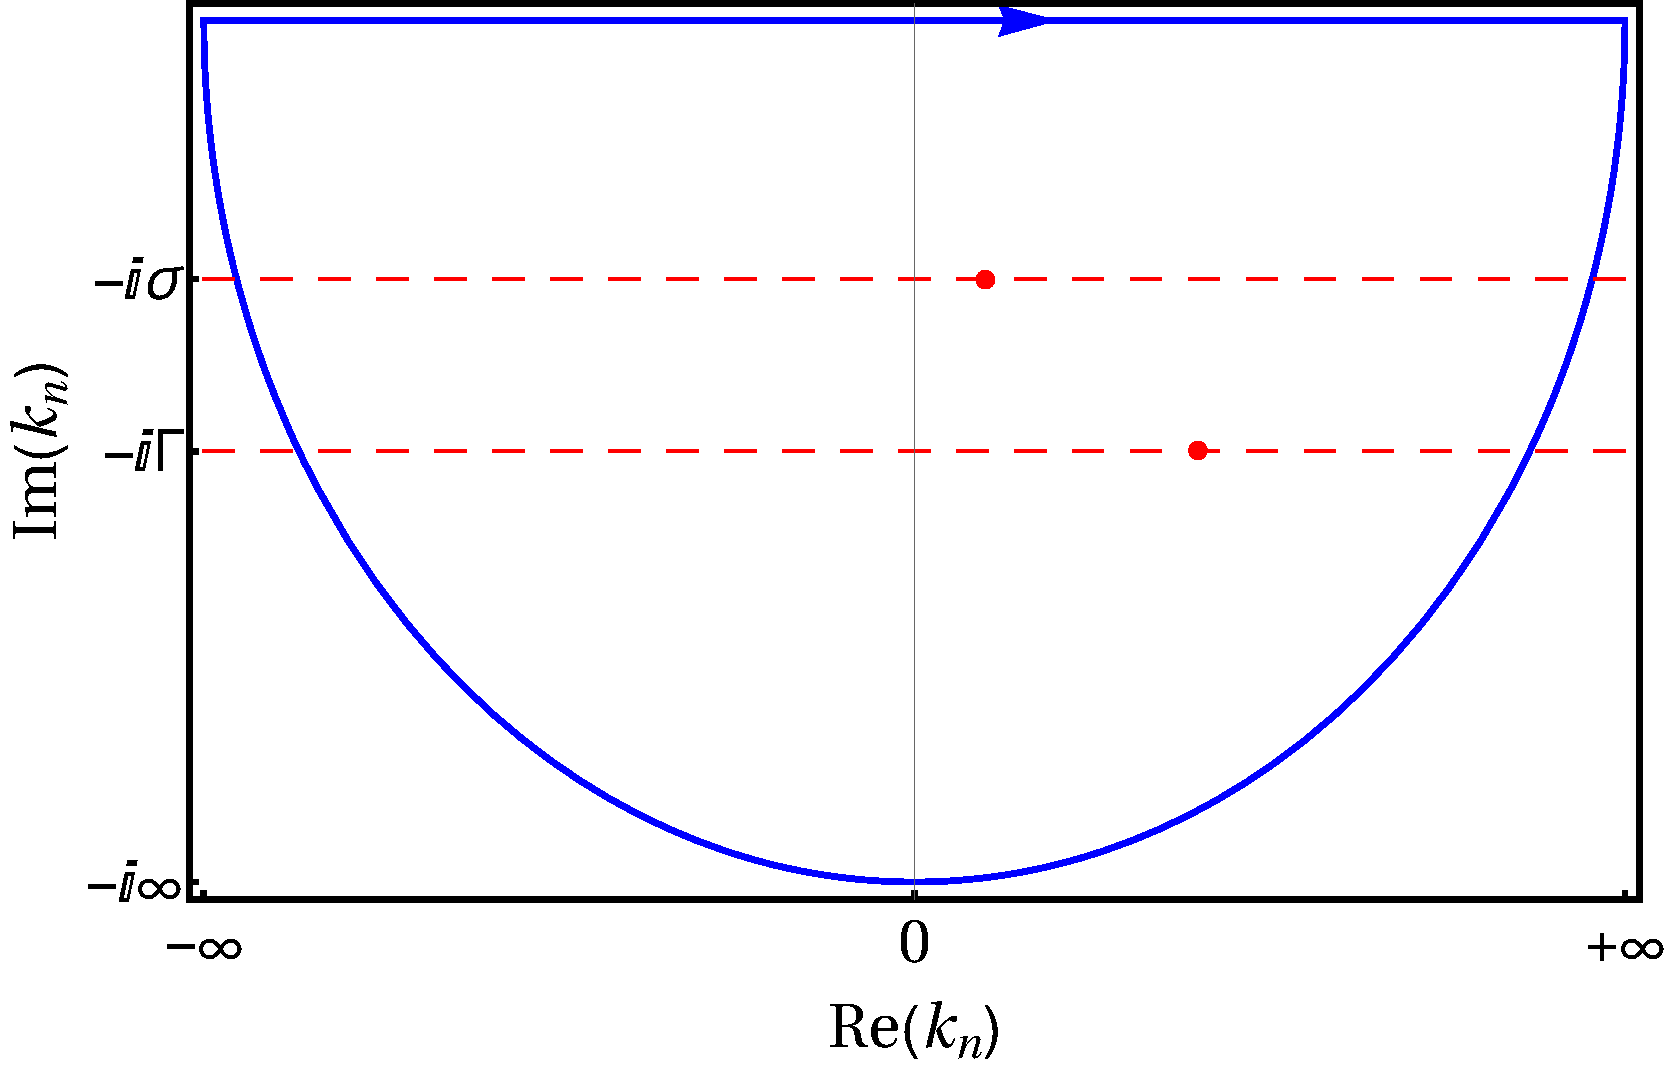
\includegraphics[scale=0.25]{lower_contour.pdf}
\caption{Integration contour for Eq. (...). The red points are the poles of the
integrand. The values of the real parts are arbitrary.}
\label{fig:lower}
\end{figure}

\begin{figure}[tbh!]
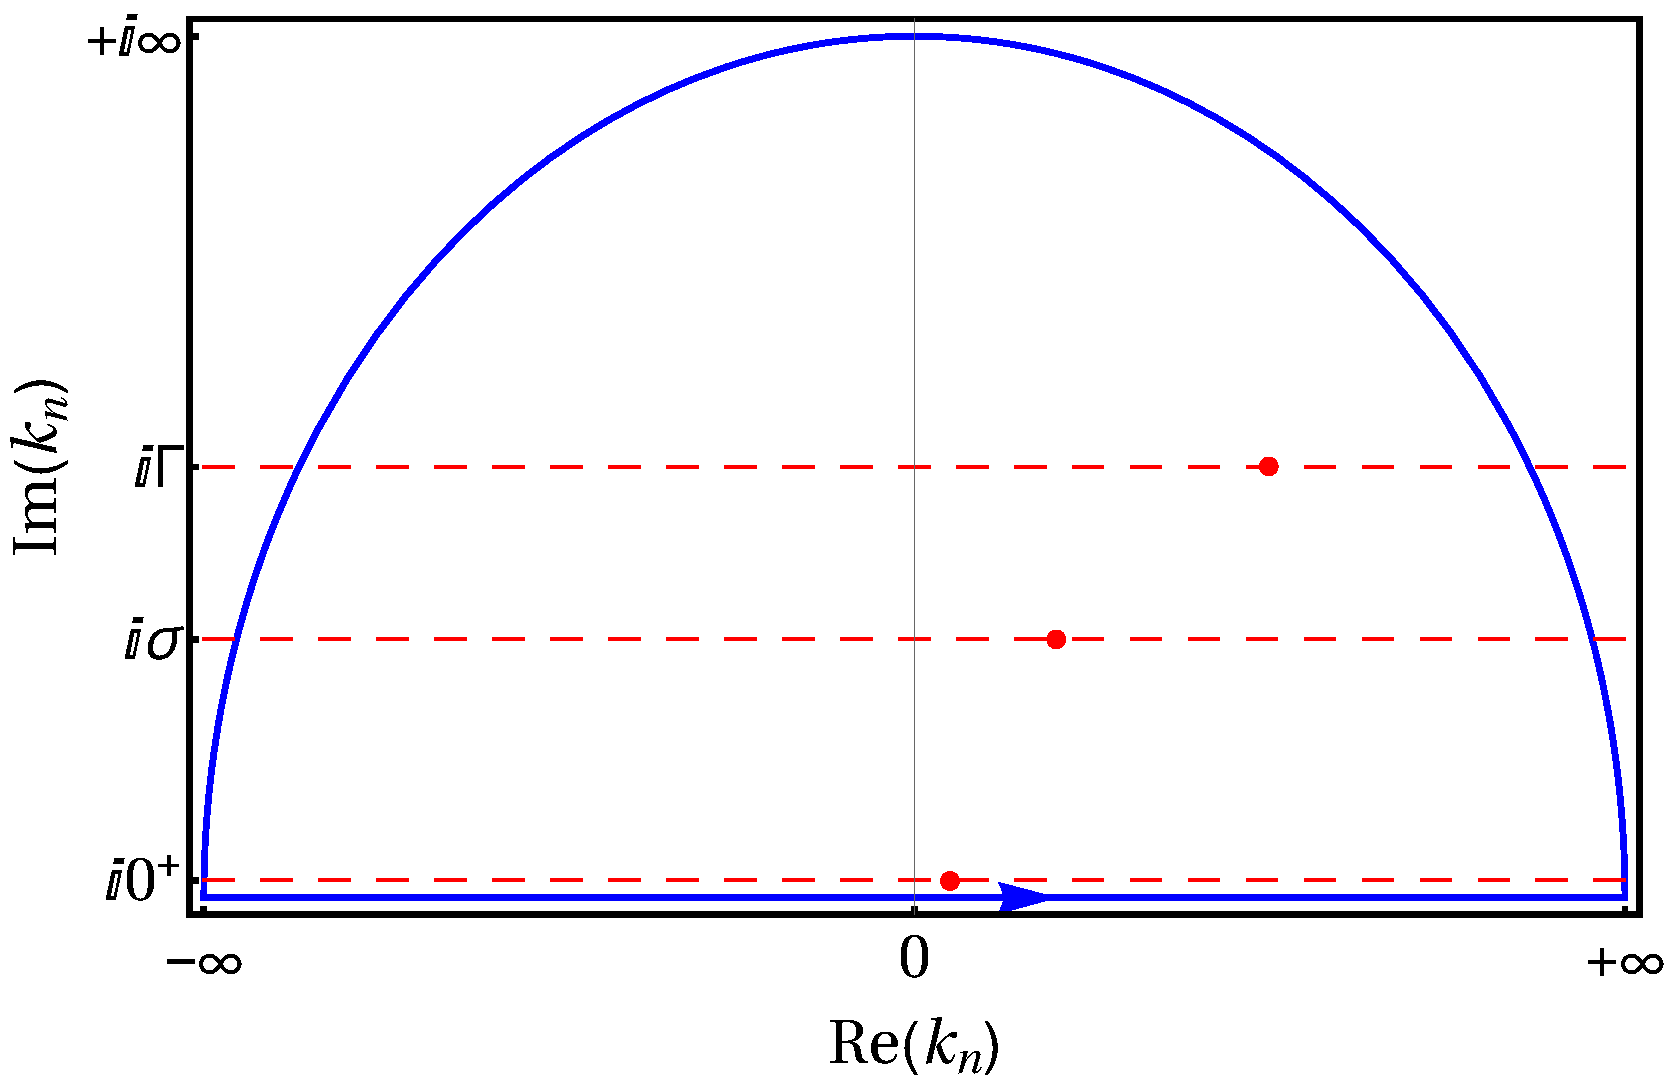
\includegraphics[scale=0.25]{upper_contour.pdf}
\caption{Integration contour for Eq. (...). The red points are the poles of the
integrand. The values of the real parts are arbitrary.}
\label{fig:upper}
\end{figure}


\section{Matrix Product States}

{\color{blue}
Brief summary of MPS and how to apply them to few-photon photonics problems.}

\bibliographystyle{apsrev4-1}
\bibliography{bib_cluster}



\end{document}